\documentclass[12pt]{article}

\usepackage{latexsym}
\usepackage{amssymb}
\newcommand{\bp}{\mbox{\rm\bf p}}
\newcommand{\be}{\begin{eqnarray}}
\newcommand{\ee}{\end{eqnarray}}
\newcommand{\bnu}{\mbox{\boldmath$\nu$}}

\newcommand{\ben}{\begin{eqnarray*}}
	\newcommand{\een}{\end{eqnarray*}}
\newcommand{\nn}{\nonumber}
\usepackage{graphicx}
\usepackage{color}

\newcommand{\N}{\mathbb{N}}
\newcommand{\D}{\mathbb{D}}
\newcommand{\T}{\mathbb{T}}
\newcommand{\A}{\mathbb{A}}
\newcommand{\B}{\mathbb{B}}
\newcommand{\G}{\mathbb{G}}
\newcommand{\F}{\mathbb{F}}
\newcommand{\R}{\mathbb{R}}
\newcommand{\W}{\mathbb{W}}
\newcommand{\V}{\mathbb{V}}
\newcommand{\U}{\mathbb{U}}
\newcommand{\J}{\mathbb{J}}
\newcommand{\Zg}{\mathbb{Z}}
\newcommand{\Gtheta}{\mathbb{\Theta}}
\newcommand{\Gphi}{\mathbb{\Phi}}

\begin{document}
\thispagestyle{empty}

\newcommand{\xe}[2]{|\!|\!| #1 |\!|\!|_{#2}}

\mbox{ }
\vspace{1cm}

\noindent {\bf Authors' report  on the revision of\\
``A Direct Imaging Method for Half-Space Inverse Elastic Scattering Problems''} \\
by Z. Chen and S. Zhou \vspace{1cm}

We are very grateful to both referees for their constructive comments. We revised the manuscript according to the suggestions of the referees. Please find below the detailed description of the changes made according to the comments.

\bigskip\noindent
{\bf 1. Changes made according to the comments of Referee 1:}

\bigskip
1) The referee said: "A main tool for these quite technical estimates is the Van de Corput result cited in Lemma 2.4. Unfortunately it is not always clear at least to me, whether all requirements for an application are satisfied. For instance the assumption $\lambda\ge 1$ in equation (3.7) or the condition $u'\ge 1$ on the whole interval $[0,\pi]$ in the proof of Theorem 3.2."

{\bf Answer}: There is a typo in the assumption of Lemma 3.5, in fact we require the assumption $\lambda\ge 1$.
This is now corrected on page 15. We notice that when $0<\lambda<1$, one has
\ben
\left|\int^b_af(t)e^{i\lambda u(t)}dt\right|\le\int^b_a|f(t)|dt&\le&\lambda^{-1}\int^b_a|f(t)|dt\\
&\le&\lambda^{-1}|b-a|\left(|f(b)|+\int^b_a|f'(t)|dt\right).
\een
Therefore, Van der Corput lemma is still valid for bounded domains when $0<\lambda<1$.

In the estimate of ${\rm III_1}$ in Theorem 3.2, we use above remark when $k_s|z-y|<1$. When $k_s|z-y|\ge 1$, we use the second part of Van de Corput Lemma in the interval where $|\cos(\theta-\phi)|\ge 1/\sqrt 2$ and the first part of Van de Corput Lemma in the interval where $|\sin(\theta-\phi)|\ge 1/\sqrt 2$ and $-\sin(\theta-\phi)$ is monotone. We have modified the proof of Theorem 3.2 on page 18 to include above considerations.

\bigskip
2) The referee said: "p4, l6: I guess, it should be �... limit of $(z + i\varepsilon)^{1/2}$ as ...".

{\bf Answer:} We have corrected. It should be the limit of $(z + i\varepsilon)^{1/2}$ for $z$ at the upper side and the limit of 
$(z - i\varepsilon)^{1/2}$ for $z$ at the lower side of the right half real axis.

\bigskip
3) The referee said: "p4, eq (2.7): $\beta$ is used twice, as summation index as well as a function."

{\bf Answer:} We have changed and denoted the function by $\varphi$ here and also throughout the paper.

\bigskip
4) The referee said: "p9, eq (2.17): a definition of $d$ is missing".

{\bf Answer:} We have corrected. In  (2.17) the integral should be the interval $(-\pi/2,\pi/2)$.
\bigskip

\bigskip\noindent
{\bf 2. Changes made according to the comments of Referee 2:}

\bigskip
1) The referee said: "They do not say what happens in the illuminated part. How they intend to use their formula so that one can indeed reconstruct this part. It is just a claim that on the illuminated part the values of the functional are non zero, maybe large, etc. Or, can they get the curvature? More?"

{\bf Answer:} We now included a discussion on the imaging function at the illuminating part under the
Kirchhoff approximation after Definition 4.1. In the illuminating part, one obtains
\ben
R_p(x_-(\theta);\tau(\theta))=-2(\lambda+2\mu)\tau(\theta),\ \ R_s(x_-(\theta);\tau(\theta))=-2\mu\tau(\theta)^\perp.
\een
Thus the imaging function is the weighted sum of the inverse of the square root of the curvature. 

From the formula after Definition 4.1, we have
\ben
\hskip0cm\hat I_d(z)&\approx&{\rm Im}\sum^2_{j=1}\int_{\Gamma_D}\left[
\int^\pi_0\overline{\tilde A_j(\theta)}\i k_pR_p(x;\tau(\theta))e^{\i k_p(x-z)\cdot\tau(\theta)}d\theta\right]\cdot\overline{\F(z,x)}e_j ds(x)\\
\hskip0cm&+&{\rm Im}\sum^2_{j=1}\int_{\Gamma_D}\left[
\int^\pi_0\overline{\tilde B_j(\theta)}\i k_sR_s(x;\tau(\theta))e^{\i k_s(x-z)\cdot\tau(\theta)}d\theta\right]\cdot\overline{\F(z,x)}e_j ds(x).
\een
Therefore, the imaging function can be viewed as the weighted sum of the scattering coefficients around $z$ due to the property of $\F(z,x)$. One usually does not know the analytical information of the scattering coefficient as it encodes the
knowledge of the scattering operator. 

The Kirchhoff approximation is proved for the Helmholtz equation for convex obstacles in [R. B. Melrose and E. T. Michael, Near peak scattering and the corrected Kirchhoff approximation for a convex obstacle, Advances in Mathematics 55 (1985): pp. 242-315]. We are not aware of any similar discussion for the elastic waves. We did some numerical simulation which indicates Kirchhoff approximation is indeed a reasonable approximation even for not very large frequency. Figures 1-3 show the comparison of scattering coefficients by using 
the numerical (Nystr\"om) method and the Kirchhoff approximation for a pear shaped
scatterer when $\omega=8\pi$.

\begin{figure}
	\centering
	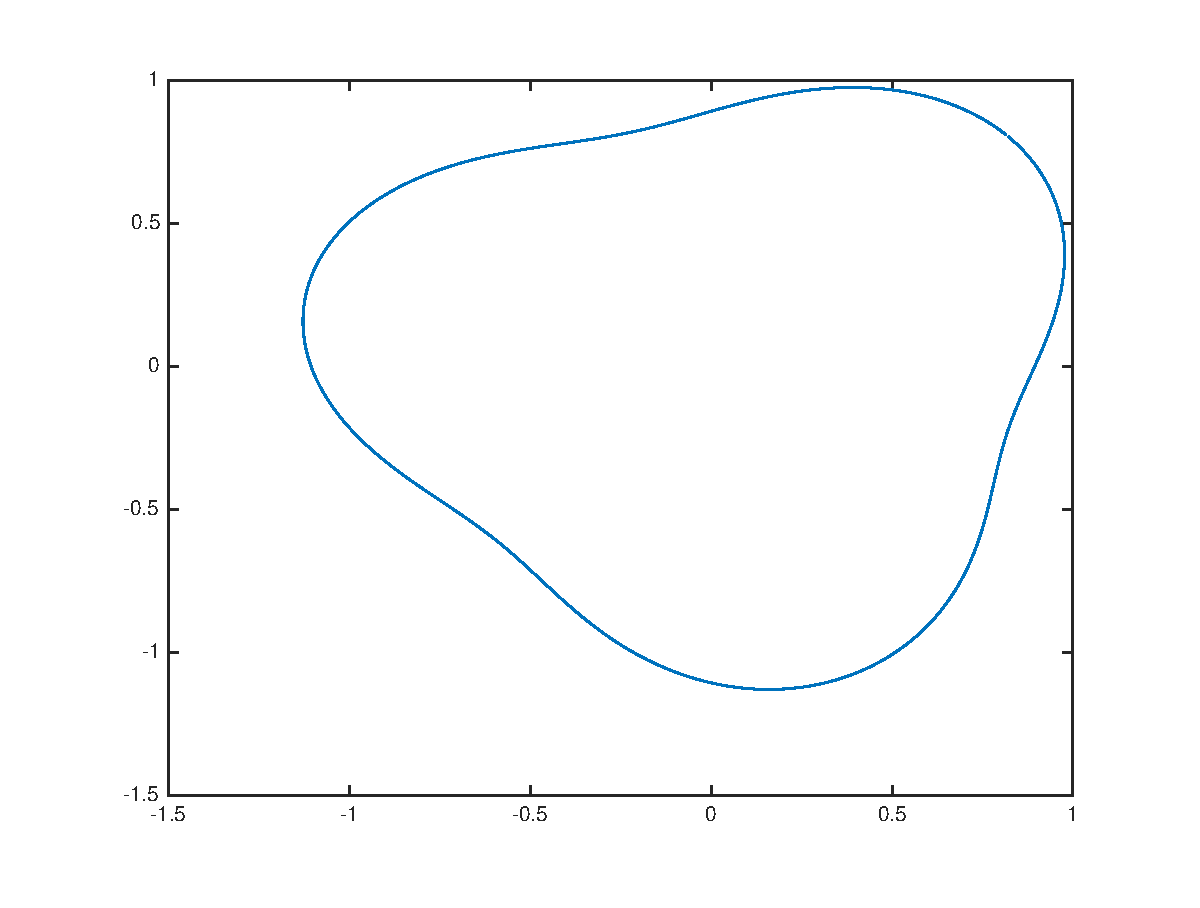
\includegraphics[width=0.48\textwidth]{./figure_sc_elastic/pear.eps}
	\caption{The pear shaped obstacle.}\label{shape}
\end{figure}

\begin{figure}
	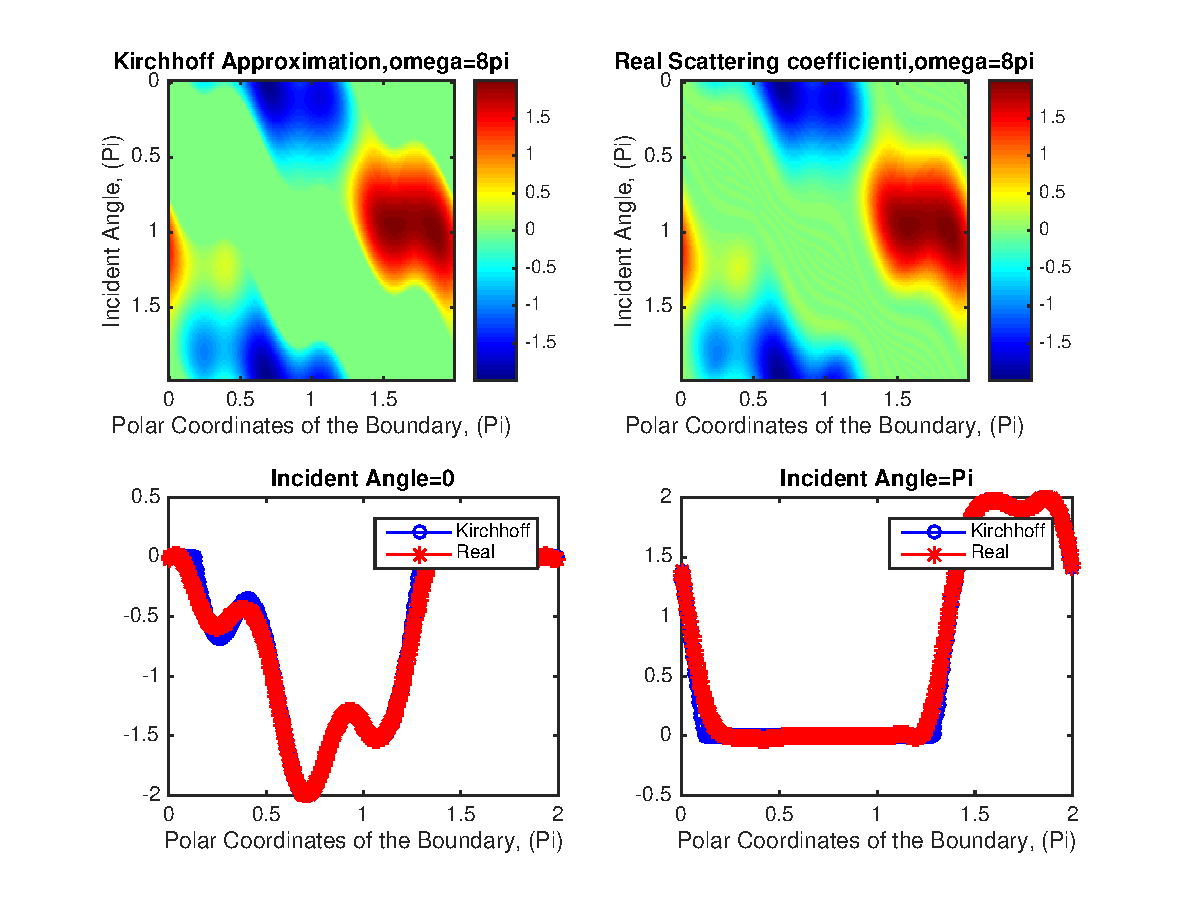
\includegraphics[width=0.98\textwidth]{./figure_sc_elastic/sc_p1_pear_8.eps} \\
	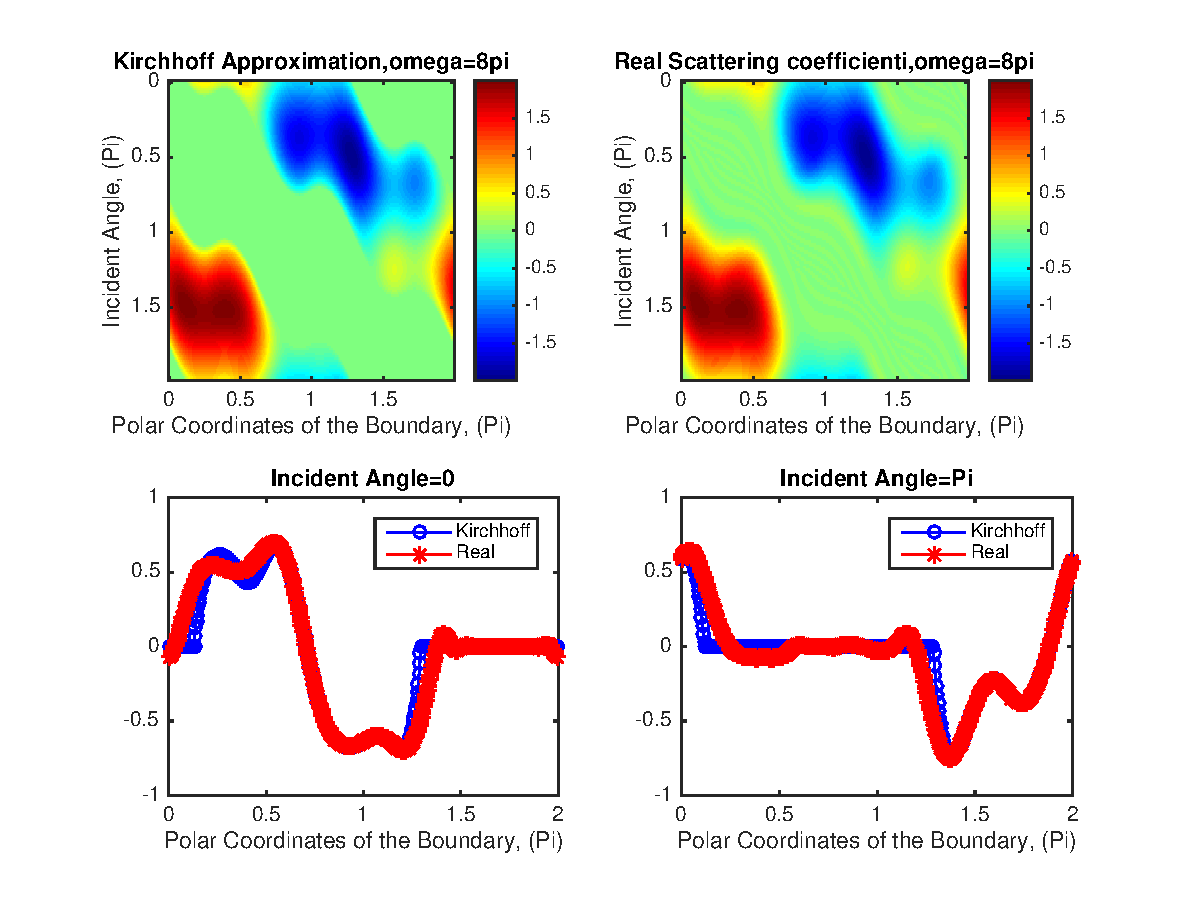
\includegraphics[width=0.98\textwidth]{./figure_sc_elastic/sc_p2_pear_8.eps}		
	\caption{The first (above) and second (below) component of the scattering coefficient and their Kirchhoff approximation for the incident $p$-wave.}
\end{figure}
	
\begin{figure}
	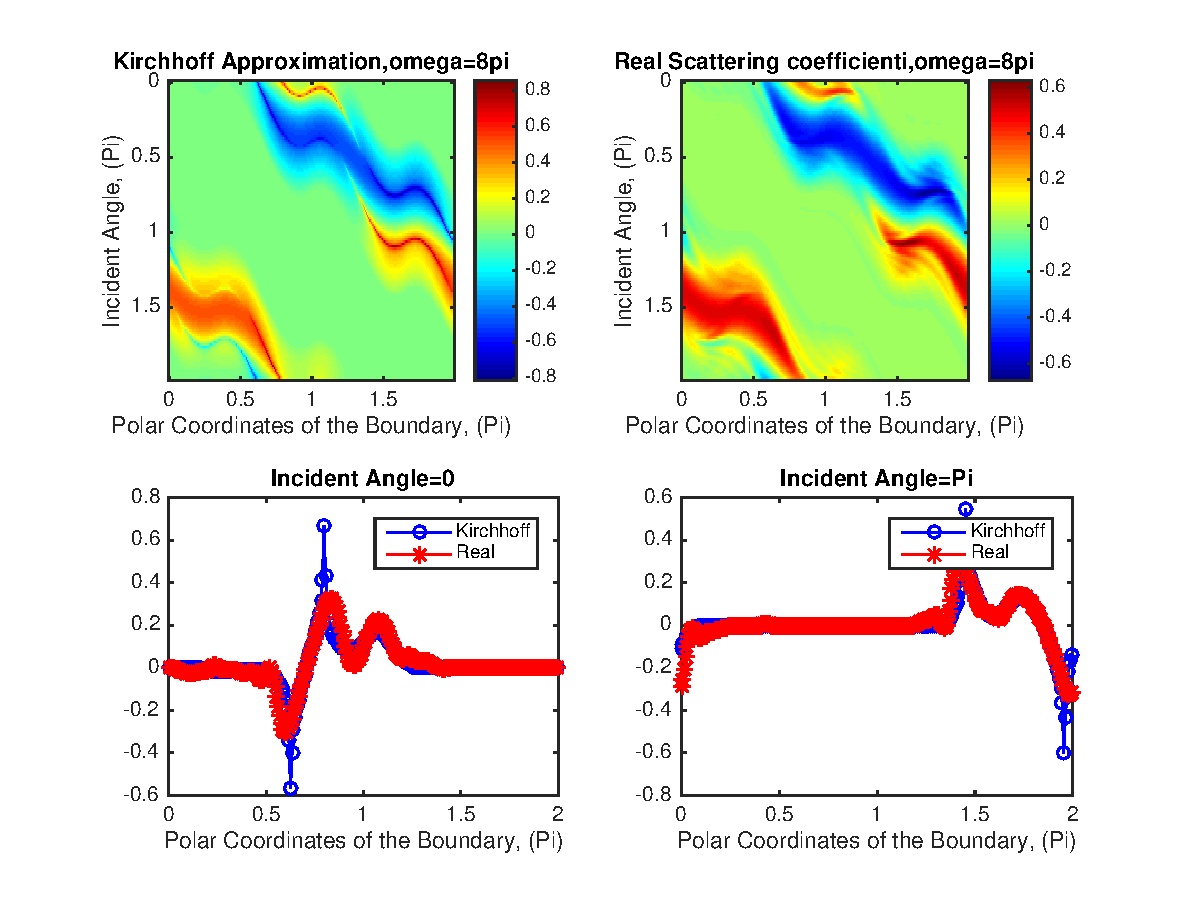
\includegraphics[width=0.98\textwidth]{./figure_sc_elastic/sc_s1_pear_8.eps}
	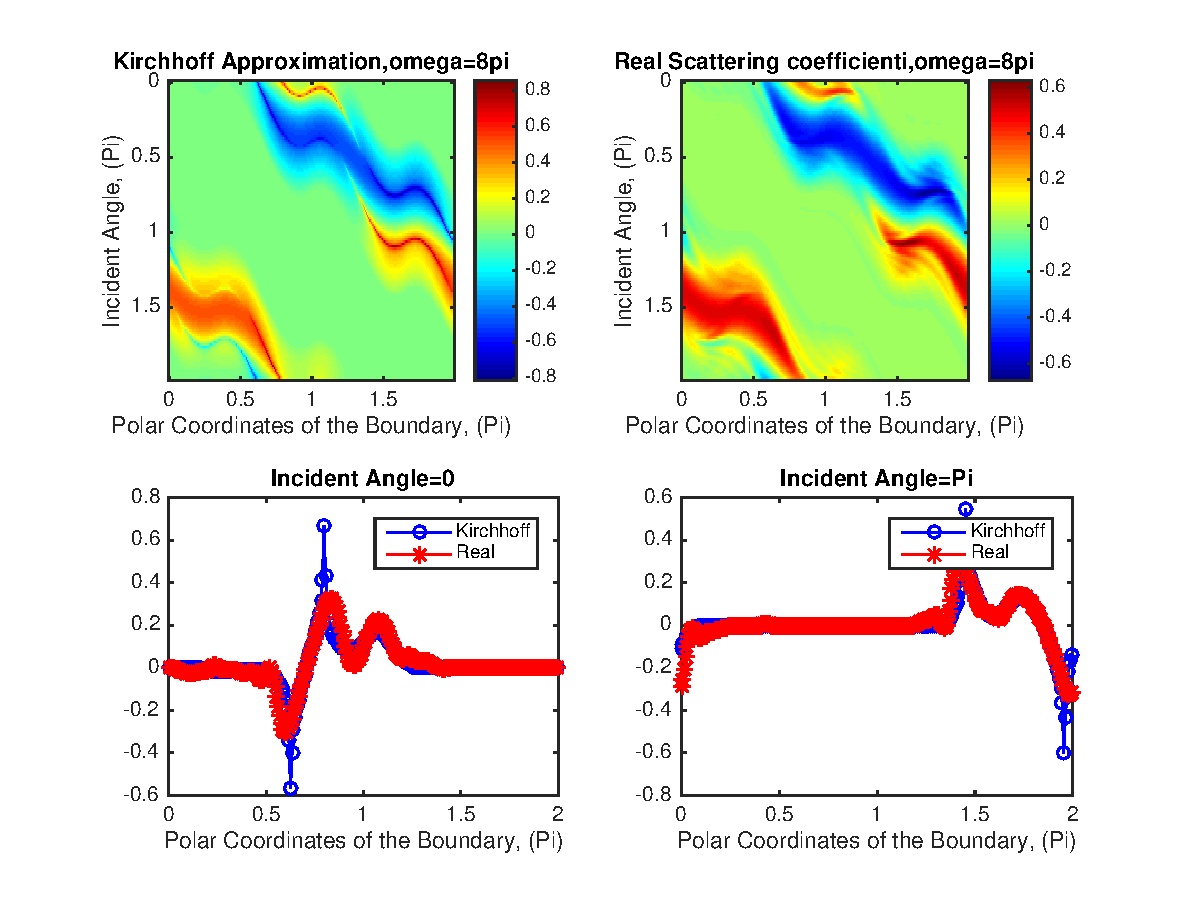
\includegraphics[width=0.98\textwidth]{./figure_sc_elastic/sc_s1_pear_8.eps}		
	\caption{The first (above) and second (below) component of the scattering coefficient and their Kirchhoff approximation for the incident $s$-wave.}
\end{figure}

\bigskip
2) The referee said: "This resolution analysis is based only on the dominating part. How about the error? Is this error small in that regime. It is not so clear. Under the already used condition, $h/d\ll 1$, the worst part of the error term is of the form
$$(k_s d_D)^3 [(h/d)^2 + (k_s h)^{-1/4}].$$
We see that one needs $(k_s)^{1/4} (d_D)^3h^{-1/4}\ll1$. However, as $k_s\gg 1$ due to Kirchhoff high-frequency approximation, this means that one needs $(d_D)^3 h^{-1/4}\ll 1$. Hence the parameters $d_D$ should be very small (or h should be large). Recalling the meaning of the parameter $d_D$, this would impose the obstacle to be very small! Of course in such condition the RTM method works fine but this condition is not what the authors want to impose. In addition, for such small obstacles, Kirchhoff high-frequency regime makes little sense. The other option is that $h$ should be large. This would mean that the object might be very far from the surface where we measure the data. In this case, it would be assimilated to a small object too."

{\bf Answer:} The referee is correct that error term is small for small obstacles, e.g. when the size of the scatterer is much smaller than the wave length. We are more interested in the regime of extended obstacles, i.e. the size of the scatterer is
comparable to the probe wave length. In this case, $k_sd_D$ is $O(1)$ and our analysis shows the error is small when $k_s h\gg 1$. This regime is not covered by the previous study on the RTM method in the literature. In this vision we also included this remark in the paper on page 23.

\bigskip\bigskip
Finally, we would like to thank again the referees for the careful reading
of the manuscript and valuable comments.

\end{document}
